\PassOptionsToPackage{dvipsnames}{xcolor}
\documentclass[twocolumn, twocolappendix]{aastex631}
\received{April 1st 2024}
\shorttitle{RATRATARRATRATTS}
\shortauthors{Wagg, Tzanidakis, Hurtado \& Gilbert-Janziek}
\graphicspath{{figures/}}

\usepackage{lipsum}
\usepackage{physics}
\usepackage{multirow}
\usepackage{xspace}
\usepackage{natbib}
\usepackage{fontawesome5}
\usepackage{xcolor}
\usepackage{wrapfig}
\usepackage[figuresright]{rotating}

% remove indents in footnotes
\usepackage[hang,flushmargin]{footmisc} 

\usepackage{styles/todo_notes}

\newcommand{\placeholder}[1]{{\color{gray} \lipsum[#1]}}

% custom function for adding units
\makeatletter
\newcommand{\unit}[1]{%
    \,\mathrm{#1}\checknextarg}
\newcommand{\checknextarg}{\@ifnextchar\bgroup{\gobblenextarg}{}}
\newcommand{\gobblenextarg}[1]{\,\mathrm{#1}\@ifnextchar\bgroup{\gobblenextarg}{}}
\makeatother

\newcommand{\tauriRAT}{RATTS\xspace}
\newcommand{\radioRAT}{RRAT\xspace}
\newcommand{\binaryRAT}{RRATRATTS\xspace}

\newcommand{\rebound}{\texttt{REBOUND}\xspace}
\newcommand{\cosmic}{\texttt{COSMIC}\xspace}
\newcommand{\cogsworth}{\texttt{cogsworth}\xspace}

\newcommand{\hi}[1]{{\color{gray} #1}}

\definecolor{dark}{rgb}{0.2,0.2,0.2}
\newcommand{\darkmode}{
    \pagecolor{dark}
    \color{white}
    \hypersetup{linkcolor=yellow,urlcolor=yellow,
                anchorcolor=yellow,citecolor=yellow}
}

\begin{document}

% \darkmode{}

\title{{\Large RATRATARRATRATTS}\\ir\hi{R}adi\hi{AT}ed \hi{rat}s \hi{A}round \hi{R}otating \hi{RA}dio \hi{T}ransients \hi{R}evolving \hi{A}bout \hi{T}he \hi{R}un\hi{A}way \hi{T}-\hi{T}auri \hi{S}tar}

% affiliations
\newcommand{\UW}{Department of Astronomy, University of Washington, Seattle, WA, 98195}

\author[0000-0001-6147-5761]{Tom Wagg}
\affiliation{\UW}

\author[0000-0003-0484-3331]{Andy Tzanidakis}
\affiliation{\UW}

\author[0000-0002-3221-9395]{V Hurtado}
\affiliation{\UW}

\author[0009-0004-8402-9608]{Samantha Gilbert-Janziek}
\affiliation{\UW}

% \author{...you?}
% \affiliation{\UW}

\correspondingauthor{Tom Wagg}
\email{tomjwagg@gmail.com}

\begin{abstract}
    Astronomers have pondered the nature of Rotating RAdio Transients (\radioRAT{}). They have scrutunised the RunAway T-Tauri Stars (\tauriRAT{}). But never before have they considered \radioRAT{}s \textit{revolving about} \tauriRAT{}s (\binaryRAT). In this interdisciplinary paper, we investigate formation mechanisms for \binaryRAT{}s and the prospect of detecting irradiated rats on planets around them.

    %Neutron stars that undergo electron-capture supernovae are thought to experience weaker kicks (on the order of $30 \unit{km}{s^{-1}}$) resulting in velocities similar to ejected T-Tauri stars.
    A pulsar-main sequence binary propelled by a supernova natal kick in the vicinity of a star forming region may encounter a \tauriRAT{}. Using N-body simulations we demonstRATe that a dynamical three-body encounter between these objects could lead to the ejection of the main sequence and the formation of a \binaryRAT{}. We consider the level of irradiation that a planet orbitting the pulsar would experience from a combination of the pulsar winds and X-ray emission from the T-Tauri star. We consider how a highly specialised species of rat may evolve to survive these conditions. Finally, we ponder the ubiquitous and fundamental nature of the concept of rats in the Universe.
\end{abstract}

\keywords{April Fools, Rats, \tauriRAT{}s, \radioRAT{}s, \binaryRAT{}s, The Joy of Acronyms}

% \tableofcontents

% \Large

\section{Introduction}
Rats. For many, that word brings to mind a scurrilous, unkempt little rodent, prowling the streets of their favourite city. But not astronomers. No, they looked beyond this simple view and thought to ask the question: what more could a rat be?

Why of course, they stated, a rat could be a runaway T-Tauri star (\tauriRAT, \citealp{Sterzik+1995}), a young protostar, heartlessly ejected from its parent molecular cloud, set free into the depths of space! Later, others cried that a rat could be a rotating radio transient (\radioRAT, \citealp{McLaughlin+2006}), a rapidly spinning neutron star (NS) living as a remnant of its former self, emitting momentary radio bursts.

And now, at last, with this paper we contemplate how these rats may come together as a Rotating Radio Transient Revolving About The RunAway T-Tauri Star (\binaryRAT).

Until recently, few \tauriRAT candidates have been observed \citep[e.g.][]{Neuhauser+1996,Neuhaeuser+1997}. But with the discovery of UJT-1 in \citet{Marti+2023}, this class of object has been revived. The \tauriRAT was first proposed as an explanation for finding infant stars, isolated from their parent molecular clouds \citep{Sterzik+1995, Sterzik+1995b}. Their isolation is thought to be a result of few-body interactions between young multiple star systems in the core of collapsing molecular clouds.

In contrast, there are more than a hundred known \radioRAT{}s, as recorded in the RRATCat \citep{RRATCat} and RRATalog\footnote{Though both names are excellent, we do highlight that the RRATalog avoids mentioning cats, which could help to avoid scaring off other \radioRAT{}s in future surveys...} \citep{RRATalog}. Despite their relative abundance, these \radioRAT{}s are still viewed as ``mysterious'' \citep[e.g.][]{mysterious_RRAT}, with many potential explanations for their millisecond long bursts of radio activity.

Some might argue that the acronyms assigned to the noble \tauriRAT and \radioRAT objects are overly similar, confusing even, for the uninitiated reader. On the contrary we emphasise that the confusion you may feel is but a symptom of the awe engendered by the fundamental nature of rats in the Universe. We will elaborate further on this realisation in Section~\ref{sec:fundamental_rats}.

In this paper we bring together two disparate\footnote{dispaRATe? Conincidence? I think not.} classes of objects and consider what one could achieve through their union as a \binaryRAT. In Section~\ref{sec:rat_formation} we discuss and demonstrate a potential formation mechanism for \binaryRAT{}s. In Section~\ref{sec:radiation} we consider the radiation that a planet in a \binaryRAT system may be subjected to, and thus in what ways rats may need to evolve. We delve further into the philosophy of the fundamental nature of rats in our Universe in Section~\ref{sec:fundamental_rats} and finally draw our conclusions.

\section{\binaryRAT{} formation}\label{sec:rat_formation}

\tauriRAT{}s are thought to be ejected from molecular clouds through a series of chaotic dynamical encounters \citep[e.g.][]{Sterzik+1995}. The dense environment of a collapsing molecular cloud contains young multiple star systems which will interact frequently. These interactions can result in T-Tauri stars acquiring excess kinetic energy and escaping the molecular cloud with high velocities (on the order of 10s of $\unit{km}{s^{-1}}$)\footnote{One might wonder what \tauriRAT{}s are running away \textit{from}. The answer is of course likely cats, particularly those purring, see \citet{cats} for a further investigation.}.

The formation of a \binaryRAT system in-situ (i.e.\ formed as a binary) may prove difficult given the dramatic nature of dynamical encounters necessary to eject a \tauriRAT from a molecular cloud. We therefore postulate that a \binaryRAT may be formed \textit{dynamically}, through a 3-body encounter between a \tauriRAT and a binary containing a \radioRAT.

\subsection{Evolving a \radioRAT--MS binary}

First, we examine a potential scenario for forming a \radioRAT in a binary with a main sequence (MS) star. Given exact nature of the \radioRAT is not currently known (and that it makes my life a lot easier...), we make the simplifying assumption that every NS is a \radioRAT.

We use \cogsworth (Wagg et al.\ in prep.), an open-source tool for self-consistent population synthesis and galactic dynamics (which applies the rapid binary population synthesis code \cosmic \citep[v3.4.8,][]{COSMIC}) to simulate example evolution of a \radioRAT--MS system. We drew binaries using the \cosmic independent sampler and evolved them with default settings for $10\unit{Gyr}$ until we found a population of bound NS--MS binaries. Using \cogsworth, we automatically converted the evolution table for one such binary into the cartoon evolution shown in Figure~\ref{fig:cartoon_ms_ns}. This functionality can be applied to \textit{any} system evolved with \cogsworth.

\begin{figure}[htb]
    \centering
    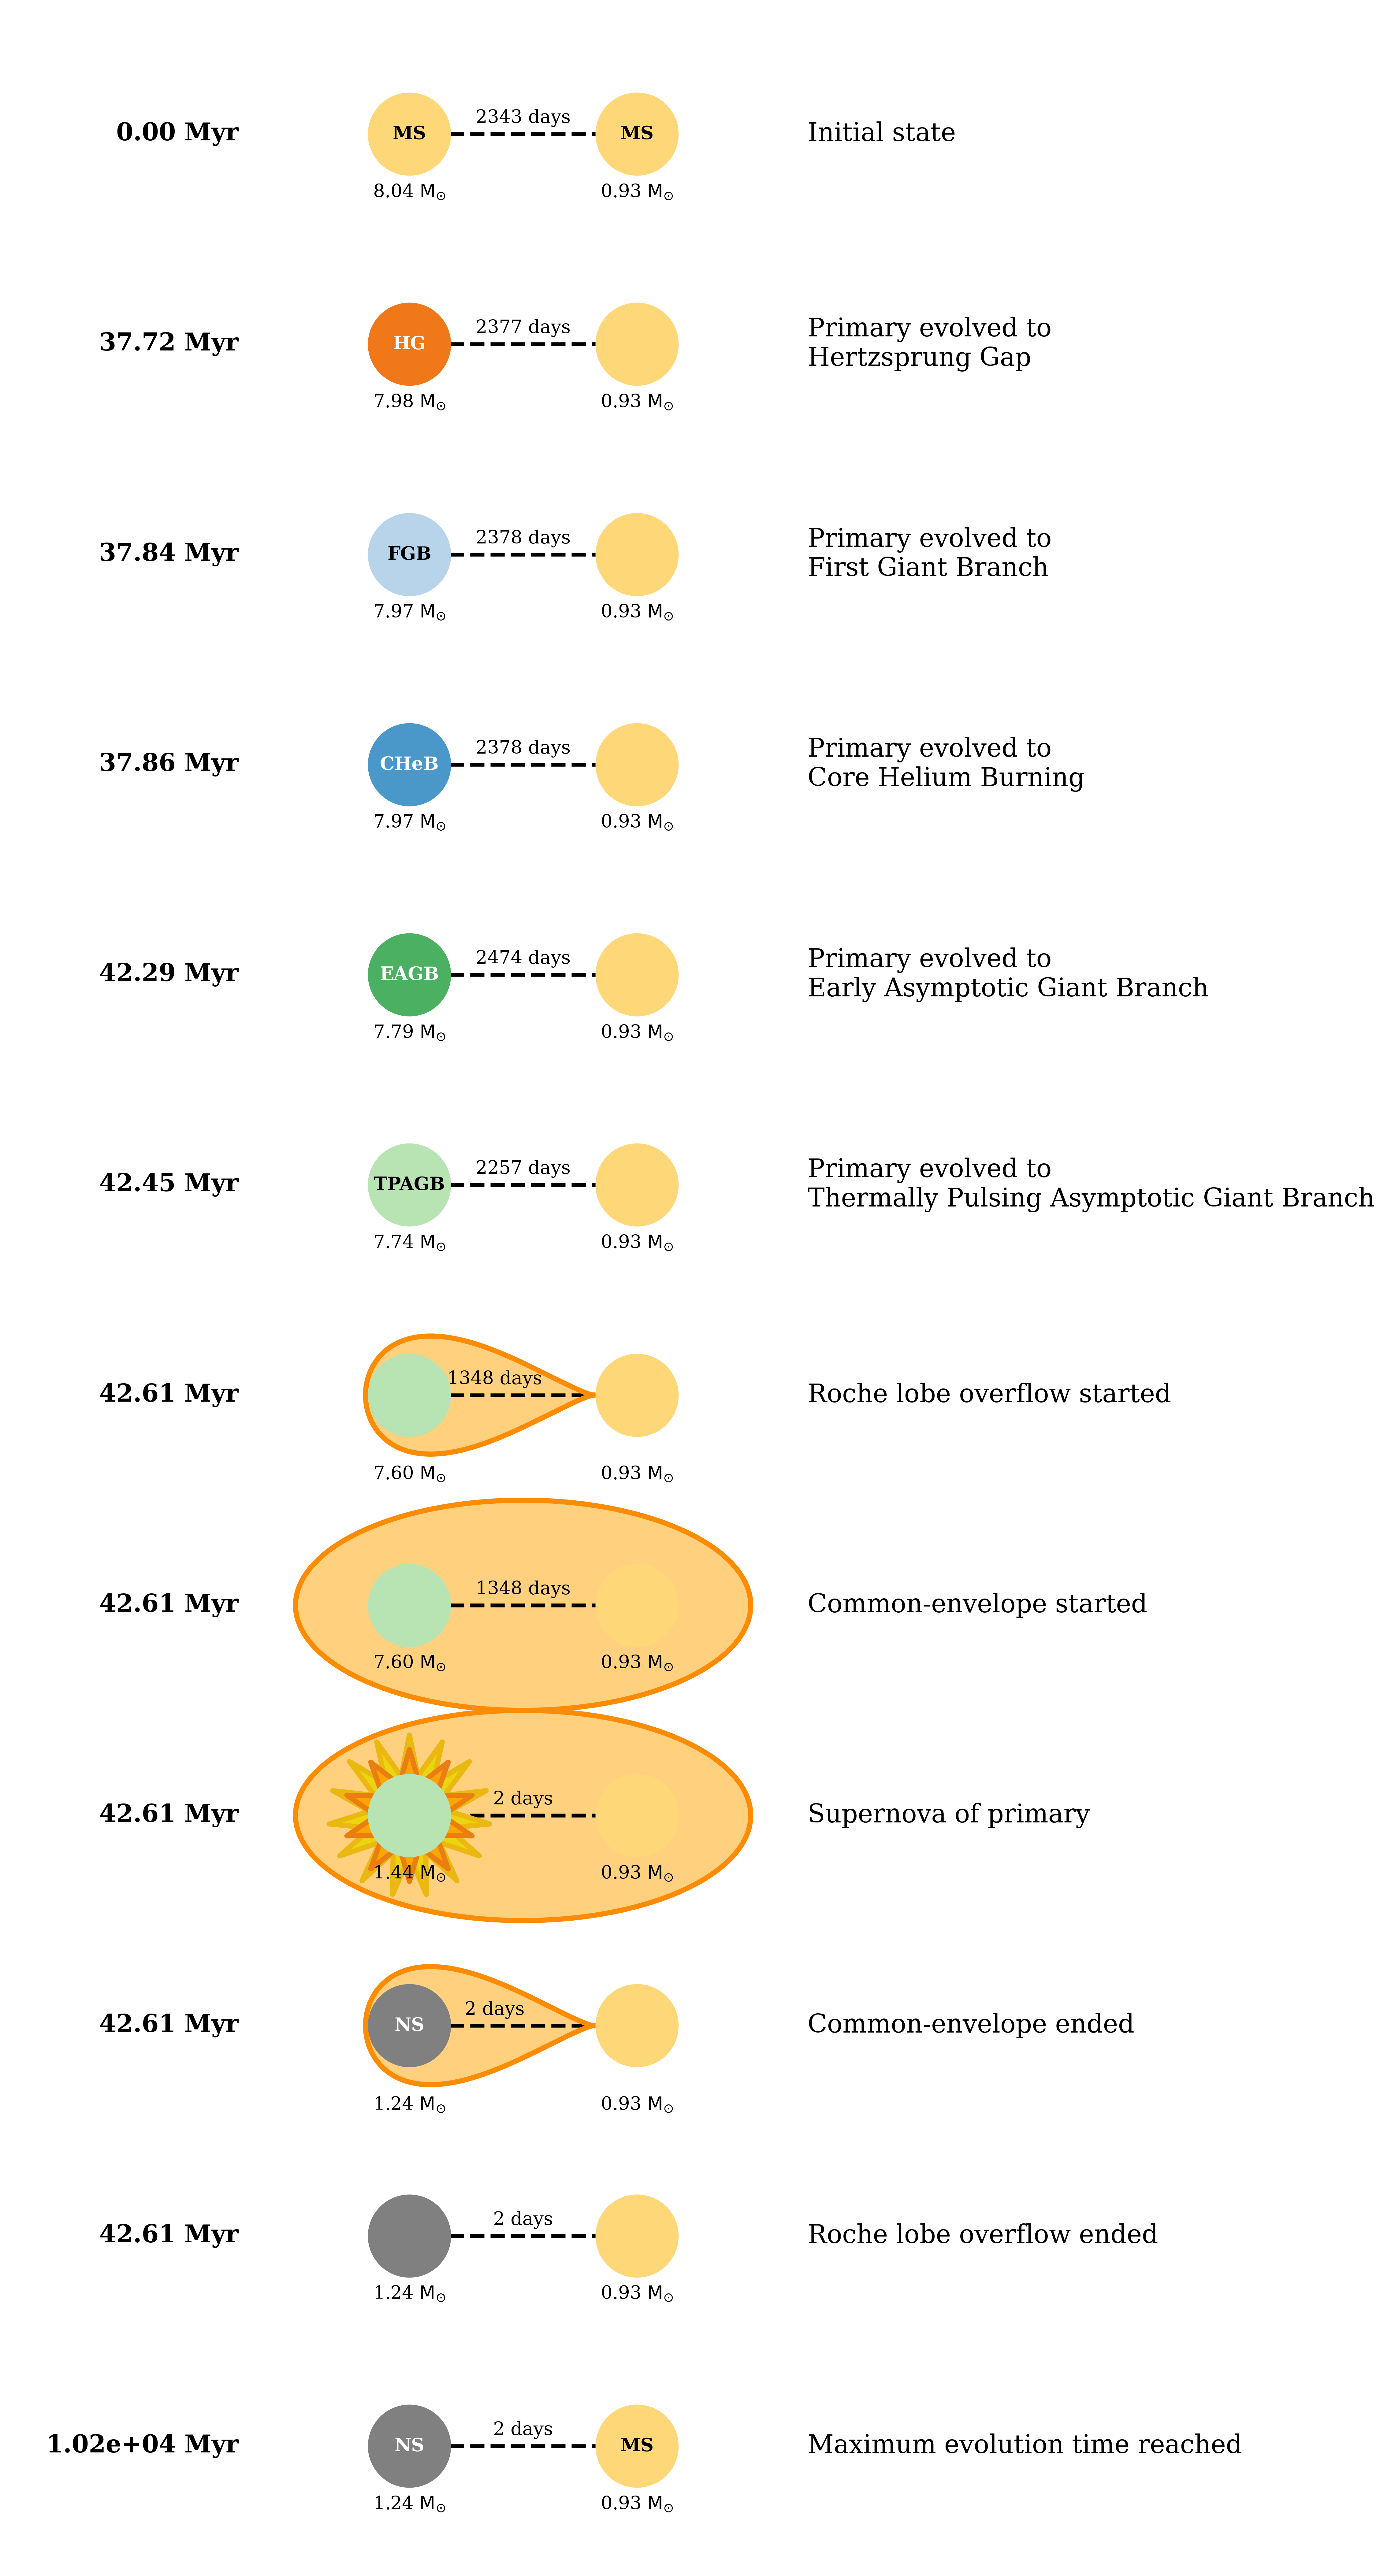
\includegraphics[width=\columnwidth]{figures/cartoon.png}
    \caption{Example evolution of a neutron star--main sequence binary through the common-envelope channel, simulated with \cosmic. \textbf{Automated visualisation achieved with \href{https://cogsworth.readthedocs.io/en/latest/}{\cogsworth}}. Each row is row represents a different evolutionary stage and is annotated with the masses of each star, orbital period and stellar type where applicable.}
    \label{fig:cartoon_ms_ns}
\end{figure}

In each row of Figure~\ref{fig:cartoon_ms_ns} we show a key stage of the evolution of the binary system. In this case, due to the low mass of the secondary star (and mass ratio of the system), it does not evolve off its main sequence on the timescale of the simulation. In contrast, the primary stars with an initial mass of ${\sim}8\unit{M_\odot}$ and evolves onto the Hertzspung Gap within $38 \unit{Myr}$ and quickly proceeds to core helium burning and the AGB phase. During this time the star loses mass due to stellar winds and its orbital period changes in tandem. During the TPAGB phase the primary overflows its Roche Lobe and leads to an unstable episode of mass transfer, resulting in a common-envelope phase, which rapidly shrinks the binary. The primary star then undergoes an electron-capture supernova, ejecting the envelope and forming a neutron star remnant. This NS-MS binary remains inert for the next $10 \unit{Gyr}$.

We highlight that the natal kick magnitude that a NS receives is likely much smaller in the case of electron-capture supernovae \citep[e.g.][]{Miyaji+1980, Gessner+2018, Igoshev+2020}, on the order of $30 \unit{km}{s^{-1}}$. These lower kicks decrease the chance of binary disruption and means that a \radioRAT--MS binary would approach a \tauriRAT-forming molecular cloud at a lower velocity, allowing for more effective 3-body encounters.

\subsection{N-body simulations of \binaryRAT{}s}

\begin{figure}[htb]
    \centering
    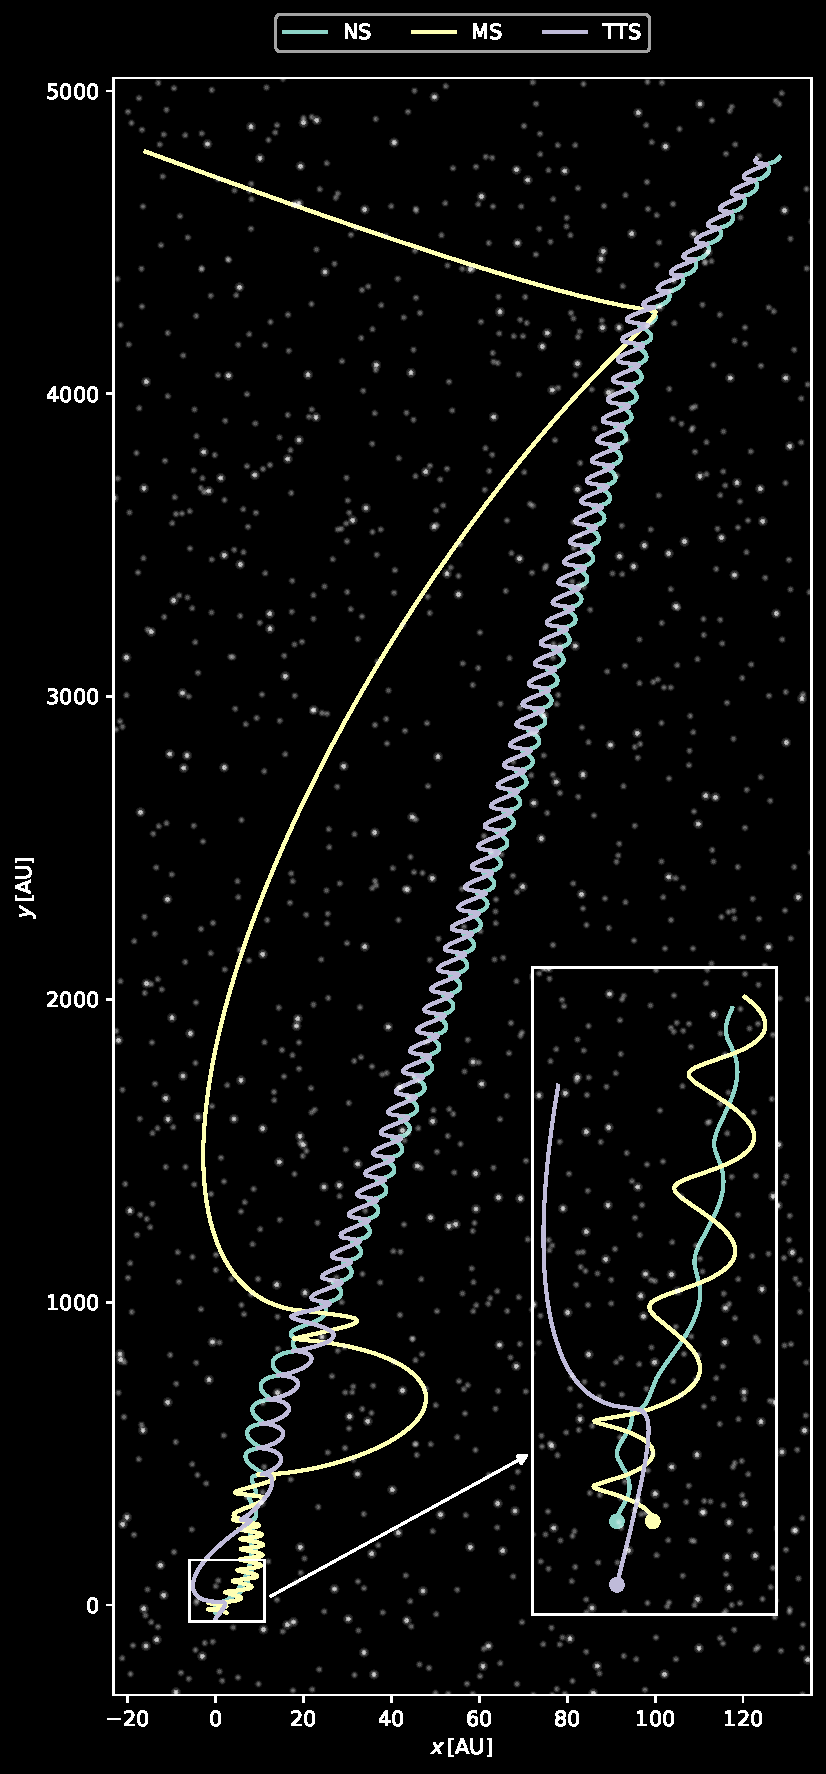
\includegraphics[width=\columnwidth]{rat_formation.pdf}
    \caption{An example formation scenario of a \binaryRAT through a 3-body exchange process between a \tauriRAT and a binary containing a main sequence star and a \radioRAT. Inset panel shows the detail of the initial evolution (with scatter points to highlight staring positions). An animated version of this plot is available \href{https://www.tomwagg.com/html/rats.html\#animated}{here}.\\\textbf{NOTE:} Of critical importance, upon rotating the image to the right (and squinting heavily), the outline of a rat is revealed (\href{https://www.tomwagg.com/html/rats.html\#annotated}{see here} for an annotated version)!}
    \label{fig:rat_rebounding}
\end{figure}

We use the N-body code \rebound\citep{REBOUND} to simulate a 3-body encounter between a \tauriRAT and a binary containing a \radioRAT and a main sequence star. We initialise a binary containing a $1.4 \unit{M_\odot}$ neutron star and $0.3 \unit{M_\odot}$ main sequence star with an orbital separation of $2.5 \unit{AU}$, moving with a centre of mass velocity of approximately $30 \unit{km}{s^{-1}}$ (motivated by the assumption that the NS underwent an ECSN). We then add a \tauriRAT of mass $0.9 \unit{M_\odot}$, moving with a velocity of approximately $45 \unit{km}{s^{-1}}$ (approximately following the characteristics of UJT-1 discovered by \citealp{Marti+2023}) towards the binary and trace the evolution of the system.

We show the evolution of this system in Figure~\ref{fig:rat_rebounding}. The process follows a typical 3-body exchange. The interaction between the \tauriRAT and initial binary leads to a series of several chaotic encounters, at the end of which the main sequence star is ejected and a \binaryRAT system is formed.

\section{Radiation and Rat Evolution}\label{sec:radiation}

We now turn our attention to rats of a more biological nature. In the following subsections we consider how a planet might form in a \binaryRAT system, how much radiation to which a planet may be subjected and how this might affect habitability. We end by postulating on how rats may evolve to deal with this.

\subsection{Pulsar planet formation scenario}

Planets around neutron stars are thought to be formed in one of three generations: (1) during the original formation of the progenitor star, (2) from the supernova fallback material that formed the NS or (3) from the material of a disrupted companion star \citep[e.g.][]{Patruno+2017}.

In the case of a \binaryRAT planets formed in the first two ways would likely be ejected from the system or disrupted during the dynamical 3-body encounter. Similarly, a \binaryRAT still has an intact companion and thus the third generation is also not possible.

We propose that, as the \binaryRAT forms, the NS may strip off some of the material from the \tauriRAT{}'s disk, which could be eventually formed into a planet in a similar manner to third-generation pulsar planets.

\subsection{Habitability of a \binaryRAT planet}

The habitability and irradiation of neutron star planets was investigated in detail by \citet{Patruno+2017}. They explain that irradiation from NSs can come from a variety of processes, including relativistic winds while the NS spins down as a pulsar, thermal emission from the surface in the form of photons and neutrinos and X-ray emission as a result of accretion of ISM material.

In addition to these sources, we also consider the additional expected X-ray emission from the companion T-Tauri star \citep{Jardine+2006}. Using the X-ray luminosity vs. mass relation from \citet{Telleschi+2007}
\begin{equation}
    \log_{10} \qty(\frac{L_X}{\unit{L_\odot}}) \approx 1.69 \log_{10} \qty(\frac{M}{M_{\odot}}) + 30.33,
\end{equation} we estimate that the X-ray luminosity of a T-Tauri star of $0.9 \unit{M_\odot}$ is $\log_{10} L_X / \unit{L_\odot} \approx 30.25$. This is on the same order as the luminosity of some pulsars considered by \citet{Patruno+2017} (see their Fig.~5), and as such may contribute to heating or stripping of the atmosphere (albeit to a lesser extent given the planet is significantly closer to the pulsar).

Following the analysis by \citet{Patruno+2017} with regards to PSR B1257+12, if we assume that part of the pulsar power is injected in the atmosphere of our theoretical planet then it \textit{may} lie within the habitable zone. This would need to be carefully balanced with X-ray radiation, including that of the T-Tauri star.

Overall, there is a chance that a planet in a \binaryRAT may lie in the habitable zone. Life on this planet may be difficult given the necessity of a thick smoggy atmosphere, dearth of visible light reaching the surface and likelihood of excess X-ray emission. Therefore, given rats survive in New York...there's no doubt they could manage this.

\subsection{Predictions for an evolved rat civilisation}
% \todo{v suggested getting grads to draw rats haha}

We now postulate on the manner in which an advanced rat civilisation may arise. As noted in the previous section, the extreme irradiation would necessitate significant evolutionary changes in rats.

We now for the first time have the chance to illustRATe the details of these evolutionary changes. In Figure~\ref{fig:horatio}, we show HoRATio, a potential first stage in evolution of these rats. The image shows him basking in the radiation of the binary system visible overhead, but additionally with a second tail that has been developed for balance whilst enjoying some pizza.

\begin{figure}
    \centering
    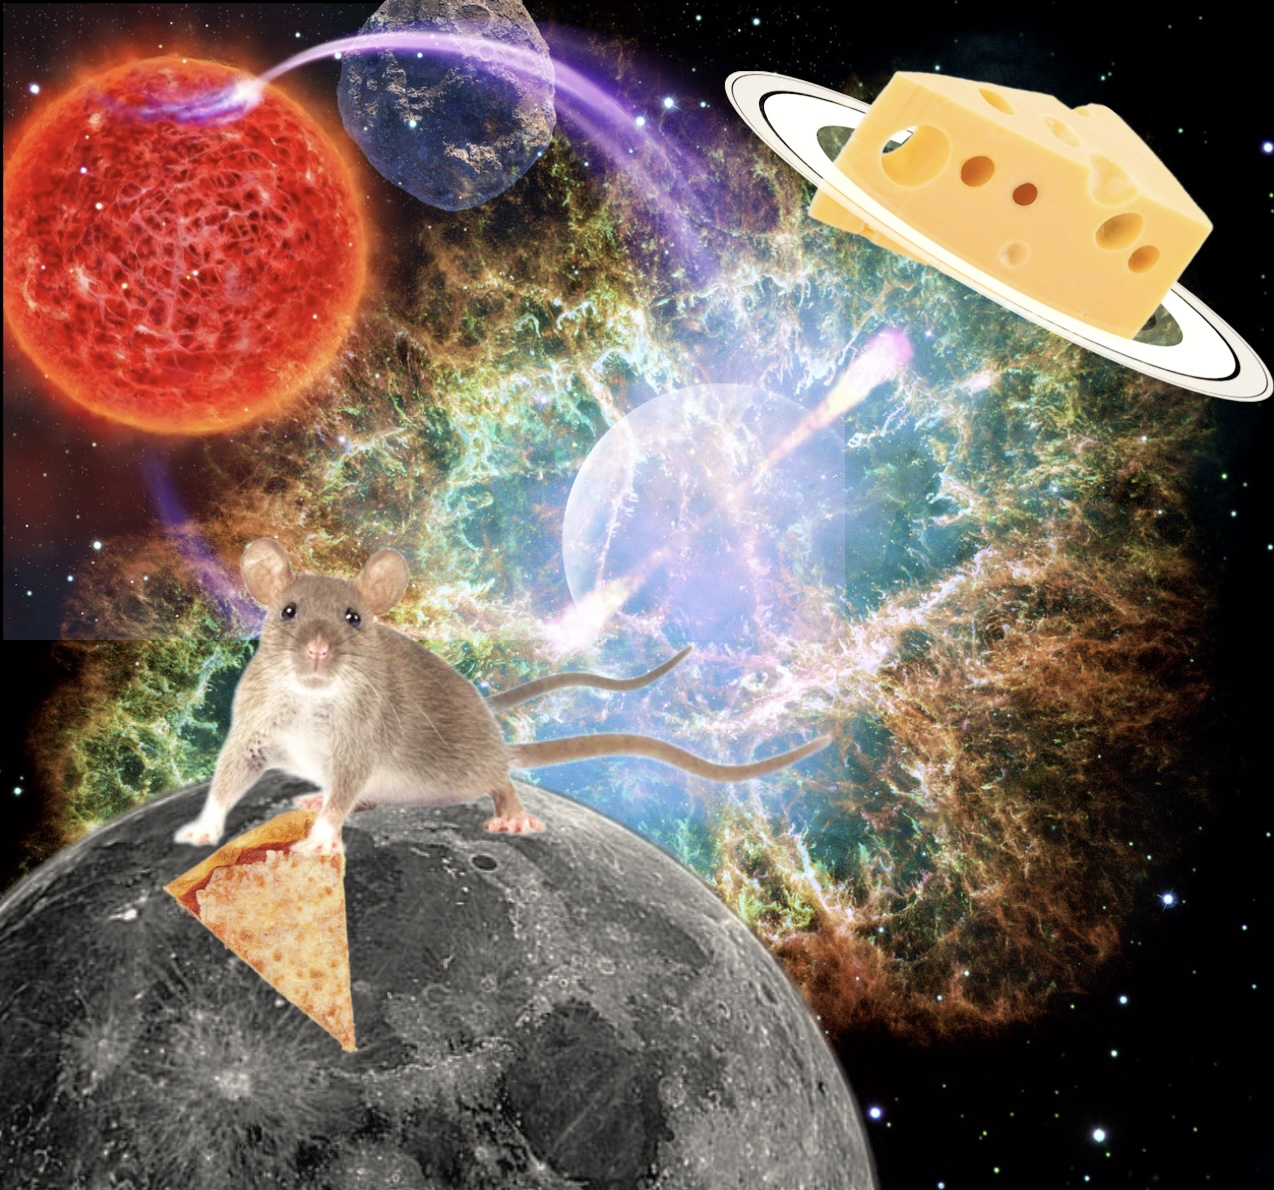
\includegraphics[width=\columnwidth]{paper/figures/horatio_updated.jpg}
    \caption{Artist's impression of the brave two-tailed HoRATio, an example of a rat that has evolved to live on the surface of hostile planets. HoRATio is shown withstanding the radiation coming from the \binaryRAT visible above. In fact, he's enjoying a slice a pizza inspired by Pizza Rat.}
    \label{fig:horatio}
\end{figure}

However, this is only the simplest case. In Figure~\ref{fig:rat-civ}, we expand upon this and consider some of the different rats that may evolve in this civilisation. In the upper left, we see a daring rat exploring the harsh environment of space. In the upper right, a rat has developed further intelligence and pursues knowledge of the Universe and the fundamental nature of rats (see Section~\ref{sec:fundamental_rats}). In the lower panels the rats have attain skills and careers, mastering the art of kaRATe and even taking on life as a space piRATe. An important corollary of Figure~\ref{fig:rat-civ} is that we clearly need more collaborations between artists and scientists.

\begin{figure*}[htb]
    \centering
    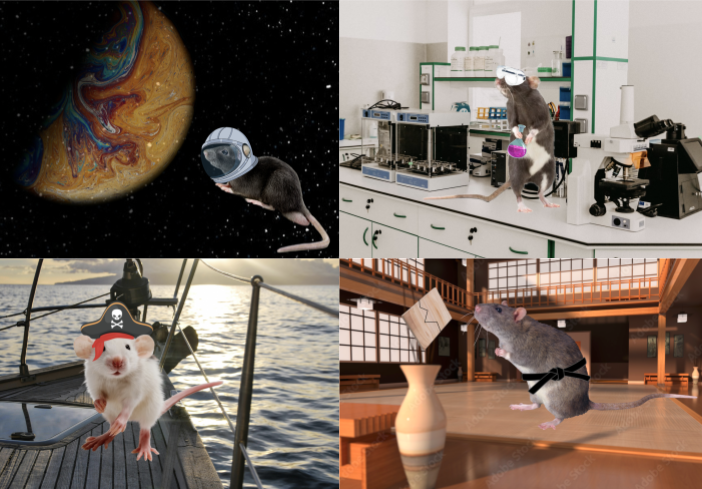
\includegraphics[width=0.75\textwidth]{paper/figures/sam_rats.png}
    \caption{Artist's impression of the civilisation of rats that may develop on a planet orbiting the pulsar in a \binaryRAT (including a rat probing new frontier of explo\textbf{RAT}ion, a PI with her own labo\textbf{RAT}ory, pi\textbf{RAT}es and ka\textbf{RAT}e enthusiasts).}
    \label{fig:rat-civ}
\end{figure*}

\subsection{Terrestrial examples of specialised rat evolution}
Though some of our claims may seem outlandish, we highlight that rats have \textit{already} demonstrated a remarkable ability to adapt to their environments through specialized evolution. Consider the humble \textbf{NYC pizza rat}\footnote{\url{https://en.wikipedia.org/wiki/Pizza_Rat}}. This rat, first observed in 2015, evolved beyond scavenging food in rubbish bins and moved on instead to human cuisine. This clearly demonstrates an ability to progress beyond simple tastes.

Beyond Pizza Rat, human imagination knows no bounds in considering other forms of potential rat evolution. Think of \textbf{Remy} the chef, of Ratatouille fame, displaying the ability to communicate, cook and even control humans. Many forget that the Teenage Mutant Ninja Turtles would just be plain old Teenage Mutant Turtles without the expert tutelage of the mutant rat \textbf{Splinter}, who displays extreme combat skills. The noble \textbf{Rattata} has evolved in size, standing at nearly half a metre tall \citep{pokemon} and terrifying anyone who comes across it. 

\section{The fundamental nature of rats}\label{sec:fundamental_rats}

As eluded to in our introduction, the prevalence of rat-based acronyms may not in fact be due to simple chance but rather the more fundamental nature of rats in our Universe. In many ways, albeit primarily orthographically\footnote{Think about it, what's ``rats'' backwards?}, rats are simply a reflection of a star and thus it is no surprise astronomer are drawn to acronyms involving them.

As yet another example of the omnipresence of rats, the sands of time are meaningless to them. Rats are present in the case of baby stars (as \tauriRAT{}s), regular stars (as boring old regular rats) and dead stars (as \radioRAT{}s), thus spanning the entire life cycle of a star.

Moreover, the ubiquity of rats is not simply restrained to astronomy. Scientists across astronomy, gastronomy, biology discover, classify and invent rats.


\section{Conclusions}%\label{sec:conclusions}
In this paper, we present new findings relating to \binaryRAT systems and their potential to host planets supporting life for irradiated rats. Though our conclusions are many and far reaching, we leave you with some of the main implications of this work:
\begin{enumerate}
    \item \textbf{Astronomers love rats}\\Whether they are running away, rotating rapidly or simply roaming the streets, astronomers cannot stop naming objects after rats.
    \item \textbf{The acronyms have gone too far folks}\\It may be time for astronomers to accept that the acronyms, and in particular back-ronyms\footnote{\url{https://en.wikipedia.org/wiki/Backronym}} are getting a little out of hand.
    \item \textbf{I should really go and work on my thesis}\\Sleep deprivation and procrastination make for powerful creative writing aids, except in the case of a thesis.
\end{enumerate}

\software{\rebound \citep{REBOUND}, \cosmic \citep{COSMIC}, \cogsworth (Wagg et al.\ in prep), Python \citep{python}, \texttt{matplotlib} \citep{matplotlib}, \texttt{numpy} \citep{numpy} }

\begin{acknowledgements}
    We are deeply grateful to Eric Agol for bringing the concept of a \radioRAT{} to our attention during a journal club presentation on \tauriRAT{} by Tom Wagg - without this critical input our insightful work might never have been realised.
\end{acknowledgements}

\newpage

\bibliography{bibs/software.bib, bibs/paper.bib}

\end{document}